\section{Neural Network Applications in Machine Translation}
\label{sect:neural-network-applications-in-machine-translation}
\textbf{NLP vs MT}: NLP covers all part up until we have a sentence. MT then takes this sentences and tries to translate it into another language.\\
Challenges of NLP:
\begin{itemize}
	\item Disambiguation: word sense, structural
	\item co-references: refering to objects within and across sentence boundaries
		\begin{itemize}
			\item anaphora: The man goes to work. He takes the bus
			\item deictic references: here, now, I, you
			\item references: same object using a synonym, hypernym
		\end{itemize}
\end{itemize}
Challenges of MT:
\begin{itemize}
	\item translation divergences: different meaning of components in different languages
		\begin{itemize}
			\item structural divergences: word order
			\item thematic divergences: changes of grammatical role
			\item head switching: ??
			\item lexicalization: swim arcoss -> to cross swimming
			\item categorial: a little bread -> un poco de pan
			\item collocational: make a decision -> eine Entscheidung treffen
		\end{itemize}
	\item translation mismatches: En: fish -> Spa: pez, pezcado
\end{itemize}

\subsection{Conventional Statistical MT}
\label{ssect:conventional-statistical-mt}
The conventional statistical MT learns automatically from the data by breaking the big problem into smaller problems. MT: Tranlation models, language models, reordering.
\begin{figure}[h]
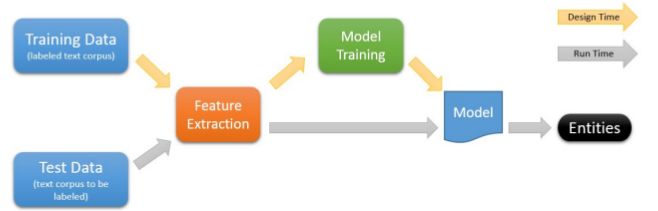
\includegraphics[scale=0.6]{conventional-statistical-MT}
\end{figure}
\begin{figure}[h]
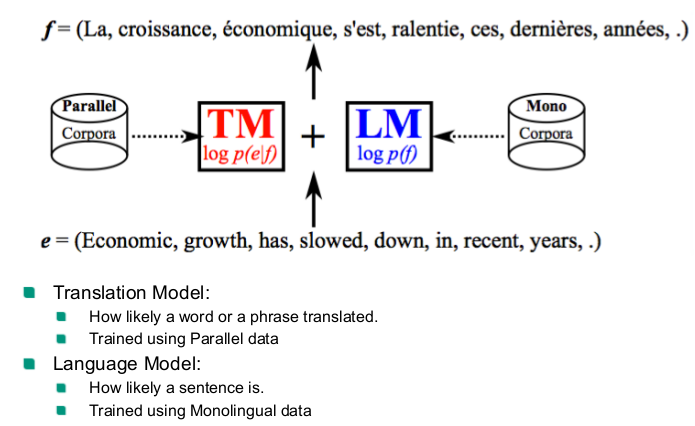
\includegraphics[scale=0.4]{statistical-mt}
\end{figure}
Problems:
\begin{itemize}
	\item requires in-depth expertise
	\item limited ability to generalize
	\item simple learning methods: cannot model well
\end{itemize}

\subsection{Neural MT}
\label{ssect:neural-mt}
Idea: train model to represent source sentence and generate target sentence from source representation.\\
\textbf{Encoder}: read input, represent content in hidden fix dimension vector (LSTM-based model):
\begin{figure}[h]
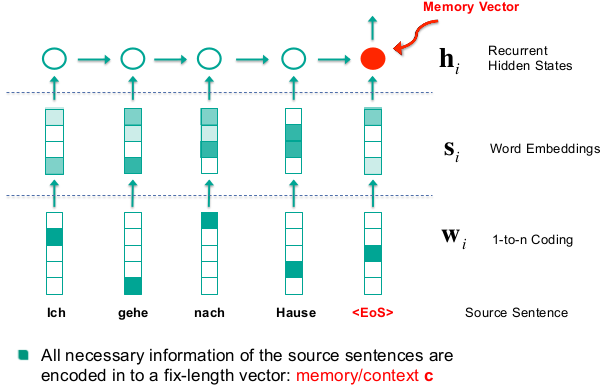
\includegraphics[scale=0.4]{encoder}
\end{figure}
\textbf{Decoder}: generate output, use fix dimension vector as input:
\begin{figure}[h]
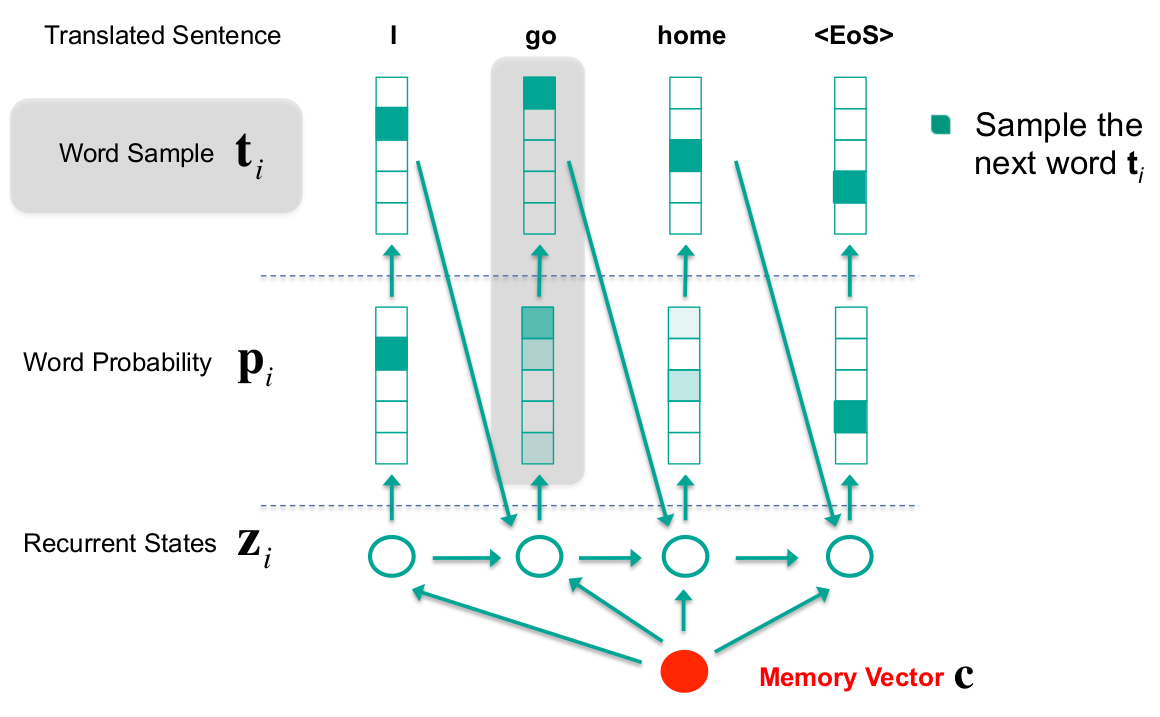
\includegraphics[scale=0.4]{decoder}
\end{figure}
Attention mechanism to set focus on important pars:
\begin{figure}[t]
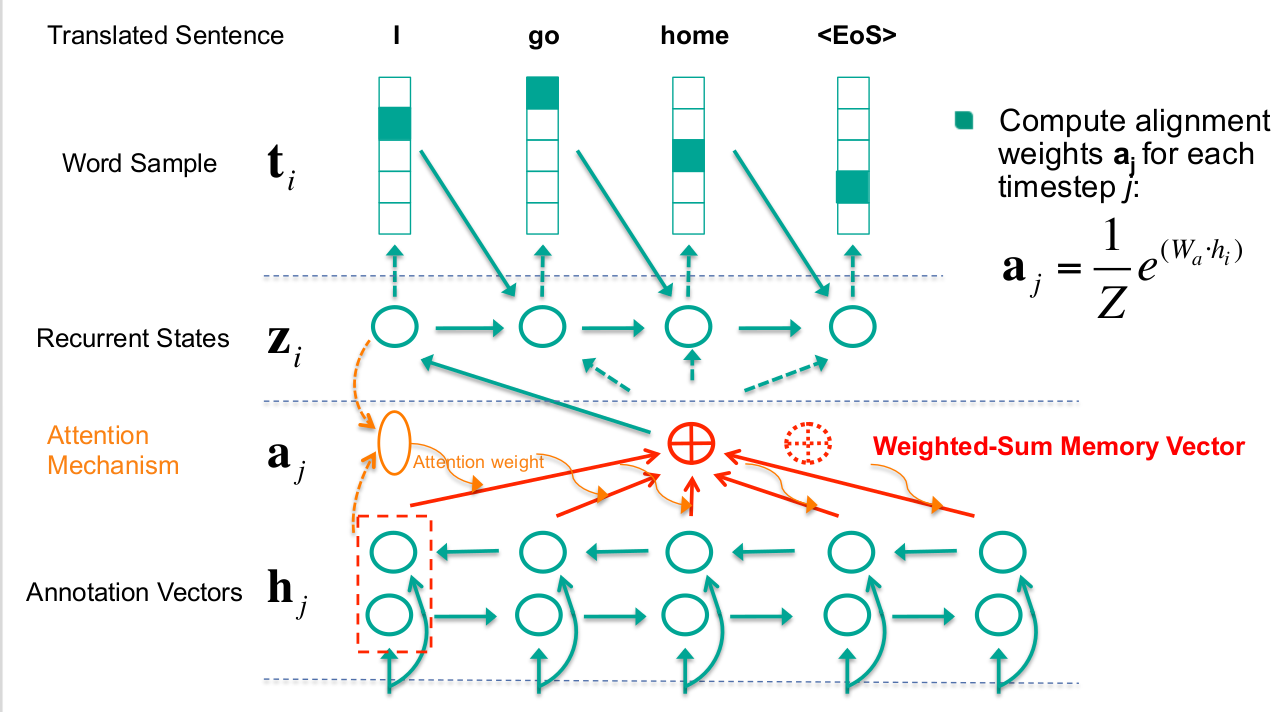
\includegraphics[scale=0.4]{attention-mechanism}
\end{figure}\\
Context vector: Represent source sentence with focus /attention on
some part of the sentence
\[
c_i = \sum_{j=1}^{T_x} \alpha_{ij}h_j
\]
Attention: Probability that this part of the source sentence is important (based on energy function)
\[
\alpha_{ij} = \frac{e^{eij}}{\sum_{k=1}^{T_x} e^{e_{ik}}}
\]
Energy function:
\[
e_{ij} = a(s_{i-1}, h_j)
\]
Bi-directional Recurrent Encoder (BiRNN):look similar to te normal RNN but the hidden state go in both directions. Two hidden states are concatenated by the \textit{annotation vector}.\\[1cm]
Encoder-Decoder-Training: the source sentence is an an english sentence, the target sentence is a german sentence. We use mini-batch training (like 100 sentences) and average the update! We can also calculate all update from all sentences in parallel. However we might have different sentence length.\\
\begin{figure}[h]
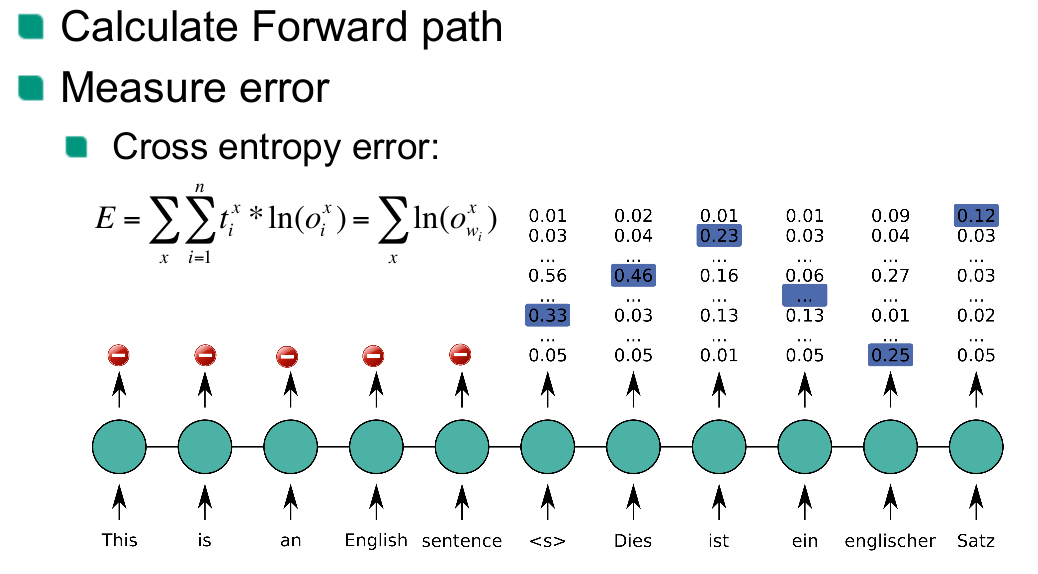
\includegraphics[scale=0.4]{edtraining}
\end{figure}
Sentence probability:
\[
p(e|f) = \Pi_{j=1}^n p(e_j|f, e_1^{j-1}
\]
Translation:
\begin{itemize}
	\item Calculate output probabilities
	\item Select best n translations
	\item Extend all hypothesis in beam
	\item Prune hypothesis not in beam
\end{itemize}
\newpage